% !TeX encoding = UTF-8
% !TeX program = pdflatex
% !BIB program = biber

% Template Revision:
% Rev. C2 -- 2021-05-11 -- Ali Varli
% Rev. C1 -- 2021-03-22 -- Ali Varli
% Rev. B1 -- 2019-11-05 -- Ali Varli

%% HINWEISE:
%% MAIN.tex ist die Hauptdatei. Hier sind sämtliche Pakete eingebunden und die allgemeine Struktur ist hier festgelegt. Im Allgemeinen müssen hier keine Änderungen vorgenommen werden.
%% In der eingebundenen Datei config.tex müssen Änderungen vorgenommen werden, die in der Datei näher erläutert sind.
%% Das Deckblatt wird mit der Datei cover/coversheet.tex eingebunden. Hier sollten keine Änderungen vorgenommen werden.
%% Für Text im Vorspann (vor der Inhaltsangabe, z.B. für Vorwort, Abstract etc.) ist die Datei frontmatter.tex vorgesehen.
%% Für den Hauptteil ist die Datei mainmatter.tex vorgesehen.
%% Das Literaturverzeichnis ist die eingebundene Datei literature.bib.
%% Die erzeugt Ausgabe ist PDF/A-1B-kompatible. Daher ist u.a. das Einbetten von transparenten Objekten (z.B. PNG mit transparentem Hintergrund) nicht erlaubt.
%% Für Verbesserungsvorschläge bin ich gerne offen.
%% Viel Erfolg :). Linz, im Oktober 2019, Ali Varli, a_v@gmx.net.

%% PLEASE NOTE:
%% MAIN.tex is the main file. All packages are pooled here and the general structure is defined here. In general, no changes need to be made here.
%% Changes must be made in the included file config.tex. Detailed information is in the file.
%% The cover page is included with the file cover/coversheet.tex. No changes should be made here.
%% The file frontmatter.tex is provided for text in the lead text (before the summary, i.e. for the foreword, abstract, etc.).
%% The file mainmatter.tex is intended for the main part.
%% The bibliography is the included file literature.bib.
%% The produced output is PDF/A-1B-compliant. Therefore, i.a., the embedding of transparent objects (e.g. PNG with transparent background) is not permitted.
%% I am open to suggestions for improvement.
%% Good luck :-). Linz, October 2019, Ali Varli, a_v@gmx.net.

\documentclass[%
	a4paper,
	11pt,
	BCOR=10mm,
	DIV=12,
	headinclude,
	headheight=16mm,
	oneside,
	onecolumn,
	openany,
	parskip=half,
	% appendixprefix,
	% toc=flat,
	% chapterentrydots=true,
	table,
	fleqn,
	% draft
]{scrbook}

\usepackage[utf8]{inputenc}

% !TeX encoding = UTF-8
% !TeX root = MAIN.tex

\newif\ifeng
%% HINWEISE: Hier müssen folgende Einstellungen vorgenommen werden:
%% PLEASE NOTE: Select your settings here:

%% Sprache: Falls die Dokumentensprache Deutsch ist, \engtrue mit einem %-Zeichen davor auskommentieren:
%% Language: If the document language is German, comment \engtrue with a % sign in front:
\engtrue

%% Hier den Namen des Autors eingeben:
%% Enter the author’s name here:
\def\author{Dominik Jochinger}

%% Hier Informationen für den rechten Block unter dem JKU-Logo eingeben, wobei die Elemente mit einem Buchstaben jeweils für die Beschreibung und mit Doppelbuchstaben für den Inhalt sind.
%% Anzuführen bei Masterarbeit: Eingereicht von, Anfegertigt am, BeurteilerIn, Mitbetreuung.
%% Anzuführen bei Dissertation: Eingereicht von, Anfegertigt am, ErstbeurteilerIn, ZweitbeurteilerIn, Mitbetreuung.
%% Anzuführen bei strukturiertem Doktorat: Eingereicht von, Angefertigt am, ErstbetreuerIn, ZweitbetreuerIn, Mitbetreuung.
%%
%% Enter information here for the right block under the JKU logo, whereby the elements should have one letter for the heading and double letters for content.
%% To be given for master thesis: Author, Submission, Thesis Supervisor, Assistant Thesis Supervisor.
%% To be given for doctoral thesis: Author, Submission, First Supervisor, Second Supervisor, Assistant Thesis Supervisor.
\def\elementA{Author}
\def\elementAA{\textbf{\author}}

\def\elementB{Submission}
\def\elementBB{\textbf{School of Education, Department of STEM Education}}

\def\elementC{Thesis Supervisor}
\def\elementCC{Univ.~Prof.\textsuperscript{in}~MMag.\textsuperscript{a}~Dr.\textsuperscript{in}\@ \textbf{Barbara Sabitzer}}

%\def\elementD{Assistant Thesis Supervisor}
%\def\elementDD{Assist.~Prof.~Mag.~Dr.\@ \textbf{Guenter Klambauer}}

%\def\elementE{Assistant Thesis Supervisor}
%\def\elementEE{Assist.~Prof.~Mag.~Dr.\@ \textbf{G\"unter Klambauer}}

%% Hier Datum eingeben (Monat der Abgabe im Prüfungs- und Anerkennungsservice):
%% Enter the date (Month and year of submission to Examination and Recognition Services):
\def\date{June 2022}

%% Hier Ort eingeben:
%% Enter the location:
\def\place{Linz}

%% Hier Titel eingeben; steht über dem K:
%% Enter the title; it appears above the K:
\def\title{VizGraph: graphical, interactive web application for teaching graph theory in computer science education}

%% Hier den Typ der Arbeit eingeben (0: Keine Arbeit, 1: Bachelorarbeit, 2: Masterarbeit, 3: Dissertation, 4: Diplomarbeit):
%% Enter the type of paper here (0: Not Thesis, 1: Bachelor’s Thesis, 2: Master’s Thesis, 3: Dissertation, 4: Diploma Degree Thesis):
\def\type{4}

%% Hier ggf. Untertitel eingeben; stehen unter dem K (nur bei 0):
%% If necessary, enter a subtitle here; below the K (only for 0):
\def\subtitle{}

%% Hier den angestrebten akademischen Grad eingeben:
%% Enter the desired academic degree here:
\def\acadDegree{Magister der Naturwissenschaften}

%% Hier die Studienrichtung eingeben:
%% Enter the major here:
\def\study{Lehramt UF Mathematik und UF Informatik und Informatikmanagement}

%% Hier die Metadaten für das PDF eingeben (mehrere Autoren und Keywords durch \sep trennen):
%% Enter metadata for the PDF here (seperate multiple authors and keywords by \sep):
\begin{filecontents*}[overwrite]{\jobname.xmpdata}
\Title{\title}
\Author{\author}
\Subject{}
\Keywords{}
\Language{de-AT}
\Publisher{}
\end{filecontents*}


\usepackage[T1]{fontenc}
\usepackage{helvet,mathpazo}
\usepackage{microtype}
\ifeng
	\usepackage[ngerman,english]{babel}
\else
	\usepackage[english,ngerman]{babel}
\fi
\usepackage[absolute]{textpos}
\usepackage{amsmath,siunitx}
\usepackage[%
	backend=biber,
	style=numeric-comp, % authoryear
	bibstyle=numeric, % authoryear
	citestyle=numeric, % authoryear
	% maxcitenames=2,
	sorting=none, %nty
	backref=true,
	backrefstyle=none
]{biblatex}
\addbibresource{literature.bib}
\usepackage{csquotes}
\usepackage{lastpage,scrlayer-scrpage}
\pagestyle{scrheadings}
\clearpairofpagestyles

\ifeng
	\ohead*{
\includegraphics[width=3cm]{cover/jkuen}}
\else
	\ohead*{
\includegraphics[width=3cm]{cover/jkude}}
\fi

\ifoot*{\date}
\cfoot*{\author}
\ofoot*{\pagemark/\pageref{LastPage}}

\setkomafont{pageheadfoot}{\sffamily\scriptsize}
\setkomafont{pagenumber}{\sffamily\scriptsize}

\usepackage[onehalfspacing]{setspace}
\usepackage{booktabs,colortbl,xcolor}
\usepackage{graphicx,wrapfig}
\usepackage[section]{placeins} %\FloatBarrier
\usepackage{float} %[H]
\usepackage{enumitem}
\usepackage{subfiles}
\usepackage{scrhack}
\usepackage[%
	bookmarksnumbered=true,
	pdfborder={0 0 0},
	pdfa
]{hyperref}
\usepackage[a-1b]{pdfx}

% \setcounter{tocdepth}{3} %subsubsection
% \setcounter{secnumdepth}{3}

\tolerance=300
\clubpenalty=10000
\widowpenalty=10000
\displaywidowpenalty=10000

% \addtocontents{toc}{\protect\enlargethispage{2\normalbaselineskip}}
% \addtocontents{lof}{\protect\enlargethispage{2\normalbaselineskip}}
% \addtocontents{lot}{\protect\enlargethispage{2\normalbaselineskip}}

\addtokomafont{caption}{\small}
\setkomafont{captionlabel}{\small\sffamily\bfseries}

%
%%
%%%%
%%%%%%%%
%%%%%%%%%%%%%%%%
\begin{document}
%%%%%%%%%%%%%%%%

\begin{titlepage}
	\setcounter{page}{0}
	\singlespacing
\sffamily
\small
\setlength{\TPHorizModule}{1mm}
\setlength{\TPVertModule}{1mm}
\mbox{}

\begin{textblock}{97}(142,20)
	\ifeng
		
\includegraphics[width=52mm]{cover/jkuen}
	\else
		
\includegraphics[width=52mm]{cover/jkude}
	\fi
\end{textblock}

\begin{textblock}{85}(155,60)
	\begin{minipage}[t]{40mm}
		\begin{flushleft}
			\ifdefined\elementA
				{\footnotesize\elementA}
				\vskip.1mm
				\ifdefined\elementAA
					\elementAA
				\fi
				\vskip5mm
			\else
				\relax
			\fi
			\ifdefined\elementB
				{\footnotesize\elementB}
				\vskip.1mm
				\ifdefined\elementBB
					\elementBB
				\fi
				\vskip5mm
			\else
				\relax
			\fi
			\ifdefined\elementC
				{\footnotesize\elementC}
				\vskip.1mm
				\ifdefined\elementCC
					\elementCC
				\fi
				\vskip5mm
			\else
				\relax
			\fi
			\ifdefined\elementD
				{\footnotesize\elementD}
				\vskip.1mm
				\ifdefined\elementDD
					\elementDD
				\fi
				\vskip5mm
			\else
				\relax
			\fi
			\ifdefined\elementE
				{\footnotesize\elementE}
				\vskip.1mm
				\ifdefined\elementEE
					\elementEE
				\fi
				\vskip5mm
			\else
				\relax
			\fi
			\date
		\end{flushleft}
	\end{minipage}
\end{textblock}

\begin{textblock}{85}(155,260)
	\begin{minipage}[t]{40mm}
		{
			\fontfamily{ugq}
			\selectfont
			JOHANNES KEPLER\\
			\ifeng UNIVERSITY
			\else UNIVERSITÄT
			\fi
			LINZ\\
		}
		Altenbergerstraße 69\\
		4040 Linz, 
		\ifeng Austria
		\else Österreich
		\fi \\
		www.jku.at\\
		DVR 0093696
	\end{minipage}
\end{textblock}

\begin{textblock}{165}[0,1](30,140)
	\begin{minipage}[b]{120mm}
		\fontfamily{ugq}
		\fontsize{32pt}{32}
		\selectfont
		\flushleft
		\title
	\end{minipage}
\end{textblock}

\begin{textblock}{120}(30,150)
	
\includegraphics[width=44mm]{cover/arr}
\end{textblock}

\begin{textblock}{165}(30,195)
	\begin{minipage}[t]{120mm}
		\Large
		\ifeng
			\ifcase\type
				\ifdefined\subtitle
					\LARGE
					\subtitle
				\else
					\relax
				\fi
				\or Bachelor Thesis 
				\or Master Thesis 
				\or Doctoral Thesis 
				\or Diploma Thesis 
			\fi 
			\vskip1mm
			\ifcase\type 
				\relax 
			\else 
				{
					\normalsize to obtain the academic degree of
				}
				\vskip2mm 
			\fi
			\ifcase\type
				\relax 
			\else 
				\acadDegree
				\vskip1mm 
			\fi 
			{
				\normalsize 
				\ifcase\type
					\relax 
					\or in the Bachelor's Program 
					\or in the Master's Program 
					\or in the Doctoral Program 
					\or in the Diploma Program 
				\fi
			} 
			\vskip2mm
			\ifcase\type 
				\relax 
			\else
				\study 
			\fi
		\else
			\ifcase\type
				\ifdefined\subtitle
					\LARGE\subtitle
				\else
					\relax
				\fi
				\or Bachelorarbeit 
				\or Masterarbeit 
				\or Dissertation 
				\or Diplomarbeit 
			\fi 
			\vskip1mm
			\ifcase\type 
				\relax 
			\else
				{
					\normalsize zur Erlangung des akademischen Grades
				}
				\vskip2mm 
			\fi
			\ifcase\type 
				\relax 
			\else
				\acadDegree \vskip1mm 
			\fi 
			{
				\normalsize 
				\ifcase\type 
					\relax 
					\or im Bachelorstudium 
					\or im Masterstudium 
					\or im Doktoratsstudium 
					\or im Diplomstudium 
				\fi
			} \vskip2mm
			\ifcase\type 
				\relax 
			\else
				\study 
			\fi
		\fi
	\end{minipage}
\end{textblock}

\end{titlepage}


%%%%%%%%%%%%
\frontmatter

% !TeX encoding = UTF-8
% !TeX root = MAIN.tex

\ifeng 
	\chapter*{Statutory Declaration}
	I hereby declare that the thesis submitted is my own unaided work, that I have not used other than the sources indicated, and that all direct and indirect sources are acknowledged as references.

	This printed thesis is identical with the electronic version submitted.

	\vskip2cm
                          
	\place, \date       \hspace*{0pt}\hfill   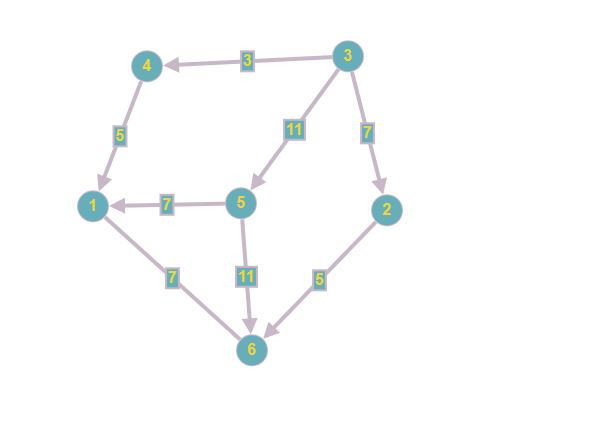
\includegraphics[width=6cm]{pics/divs/sign.JPG}



\else 
	\chapter*{Eidesstattliche Erklärung}
	Ich erkläre an Eides statt, dass ich die vorliegende \ifcase\type Arbeit \or Bachelorarbeit \or Masterarbeit \or Dissertation \or Diplomarbeit \fi selbstständig und ohne fremde Hilfe verfasst, andere als die angegebenen Quellen und Hilfsmittel nicht benutzt bzw. die wörtlich oder sinngemäß entnommenen Stellen als solche kenntlich gemacht habe.

	Die vorliegende \ifcase\type Arbeit \or Bachelorarbeit \or Masterarbeit \or Dissertation \or Diplomarbeit \fi ist mit dem elektronisch übermittelten Textdokument identisch.

	\vskip1cm
	\place, \date
\fi


\ifeng
	\chapter*{Abstract}
\else
	\chapter*{Kurzfassung}
\fi

%% Hier Abstact in der Sprache eingeben, in der die Arbeit geschrieben wurde.
%% Enter here the abstract in the main language.
In recent years the use of digital learning systems boosted rapidly. The COVID-19 pandemic led to an increase of homeschooling situations, and therefore the usage of digital technology in education\cite{Alabdulaziz}. The aim of this thesis is to develop an interactive online learning software for teaching graph theory in computer science education. Graph theory has major applications in our daily life. For example, it is used in modern navigation systems to find the shortest path to the desired destination. Computer science education should be used to teach the concepts behind new technologies. The VizGraph application follows the COOL (Computer-supported Open Learning) informatics principle\cite{SabitzerCoolinfo}\cite{SabitzerCool}. VizGraph allows students to discover graph theory interactively by drawing their own graphs. It’s a modern single page web application (SPA) to draw graphs and automatically computes and visualize properties of a graph. The use of VizGraph should encourage computational thinking and solution based learning.\\ 
The application is implemented in Typescript\cite{bierman2014understanding} and uses the modern Angular\cite{jain2014angularjs} web framework. The visualization is realized with the d3.js\cite{d3js} JavaScript library. D3.js is used to generate dynamic and interactive visualizations. The main component of the web application is a graphic editor, which is structured according to the Model-View-Controller(MVC) design pattern and applies the object-oriented (OO) programming paradigm\cite{mossenbock}.\\ 
The VizGraph application allows students to easily draw their own graphs by adding nodes and edges. The app includes the following features:
\begin{itemize}
\item add nodes (vertice)
\item add connection between nodes (edge)
\item connection can be directed or undirected with weight
\item compute adjacency matrix
\item compute incidence matrix
\item compute distance matrix 
\item find shortest path (Dijkstra algorithm)
\item find cycle
\end{itemize}
It is possible to export the graph visualization as an image or to save the graph in GeoJSON\cite{rfc7946} open standard format.
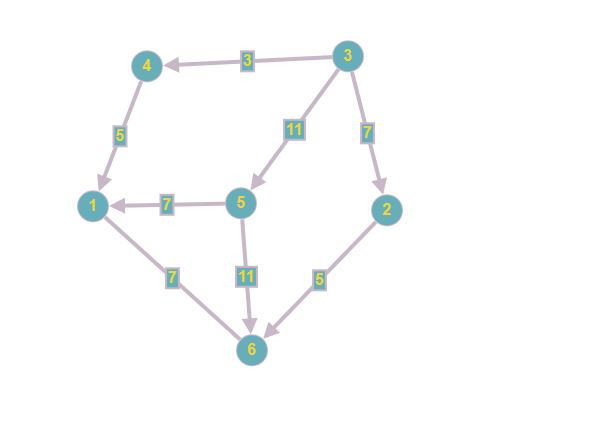
\includegraphics[width=10cm]{pics/graphen.JPG}
{
	\let\clearpage\relax
	\ifeng
		\selectlanguage{ngerman} 
		\chapter*{Kurzfassung}
	\else
		\selectlanguage{english} 
		\chapter*{Abstract}
	\fi

	%% Hier Abstact in der jeweils anderen Sprache eingeben.
	%% Enter here the abtract in the other language.
In den letzten Jahren hat sich der digitale Unterricht und die Verwendung von digitalen Lernsystemen enorm gesteigert. Die COVID-19 Pandemie f\"uhrte zu vermehrtem Homeschooling, und den damit verbundenen Einsatz von digitalen Technologien im Unterricht\cite{Alabdulaziz}. Ziel dieser Diplomarbeit ist die Entwicklung einer interaktiven online Anwendung um Graphentheorie im Informatikunterricht vorzustellen. In unserem Alltag benutzen wir oft unbewusst die Algorithmen der Graphentheorie. In modernen Navigationssystemen wird mit Hilfe der Graphentheorie der kürzste Weg zwischen zwei Orten bestimmt. Der Informatikunterricht soll nicht nur die Anwendung, sondern auch die technischen Konzepte dieser neuen Technologien vermitteln. Die VizGraph Anwendung unterst\"utzt die Sch\"uler beim Lernen nach dem COOL (Computer-supported Open Learning) Informatik Ansatz\cite{SabitzerCoolinfo}\cite{SabitzerCool}. Dabei sollen Sch\"uler spielerisch die Konzepte der Graphentheorie entdecken. Die Software ist eine moderne Single Page Web Application (SPA) und erm\"oglicht die Visualisierung von Graphen, und berechnet automatisch deren Eigenschaften. Durch das Anwenden der App soll das l\"osungsorientierte und informatische Denken der Sch\"uler best\"arkt werden.\\
Die Webanwendung ist in Typescript\cite{bierman2014understanding} programmiert, und verwendet das moderne Angular\cite{jain2014angularjs} Webframework. Die Visualisierung ist mit Hilfe der d3.js\cite{d3js} JavaScript Bibliothek umgesetzt. D3.js wird f\"ur die Erzeugung von dynamischen interaktiven Grafiken verwendet. Die Hauptkomponente der  Webanwendung ist ein Grafikeditor zum Zeichnen des Graphen. Dieser basiert auf dem Model-View-Controller(MVC) Entwurfsmuster und ist objektorientiert(OO) programmiert\cite{mossenbock}.\\ 
Die VizGraph Webanwendung bietet den Sch\"ulern eigene Graphen zu zeichnen, indem sie Knoten und Kanten einfach hinzuf\"ugen. Die Anwendung beinhaltet die folgenden Funktionalit\"aten:
\begin{itemize}
\item Knoten hinzuf\"ugen
\item Kante hinzuf\"ugen
\item gerichtete oder ungerichtete Kanten mit Gewicht
\item Bestimmten Adjazenzmatrix
\item Bestimmten Inzidenzmatrix
\item Bestimmten Distanzmatrix 
\item K\"urzesten Pfad bestimmen (Dijkstra Algorithmus)
\item Kreisfreite Graphen
\end{itemize}
Die Graphen k\"onnen entweder in einer Bilddatei, oder im GeoJSON\cite{rfc7946} offenen Standardformat abgespeichert werden.
	\ifeng
		\selectlanguage{english}
	\else
		\selectlanguage{ngerman}
	\fi
}


\begin{singlespace}
	\tableofcontents
	\listoffigures 
	\listoftables
\end{singlespace}


%%%%%%%%%%%
\mainmatter

%% !TeX encoding = UTF-8
% !TeX root = MAIN.tex

\chapter{Text}

Text.
\newpage
% !TEX root = MAIN.tex
\chapter{Introduction}\label{sec:intro}
Lernen im Mathematikunterricht digital unterst\"utzen.

\section{Motivation}\label{sec:motivation}
Durch Corona Pandemie vermehrter Einsatz von digitalen Technologien im Unterricht.
Steigerung der Lernmotivation und des Lernerfolges.
Digitale Unterricht als Bestandteile eines integrativen Gesamtkonzepts.

\section{Related Works}\label{sec:works}
Vergleich mit anderen Apps:
Geogebra, Mathematica, online Tools


\section{Didactics and Curriculum}\label{sec:lehrplan}
Wo kommt Graphentheorie im Lehrplan vor. In wlecher Schulstufe behandelt. 

\newpage
% !TEX root = MAIN.tex
\chapter{Graphtheory}\label{sec:geo}


\section{Historical Remarks}\label{sec:geoobj}
K\"onigsberger Br\"ucken Problem

\section{Mathematical Graphtheory}\label{sec:works}
Mathematische Beschreibung der Graphentheorie

\newpage
% !TEX root = MAIN.tex
\chapter{VizGraph Webapp}\label{sec:geoforms}


\section{Typescript}\label{sec:typescript}
introduction to typescript

\section{Angular Webframework}\label{sec:angular}
introduction to angular

\section{Visualization with d3.js}\label{sec:d3}
introduction to d3.js

\section{VizGraph Implementation}\label{sec:geoimpl}
Design and implementation of VizGraph webapp

\newpage
% !TEX root = MAIN.tex
\chapter{Computer Science Education with VizGraph}\label{sec:geoformedu}


\section{Learning sequence}\label{sec:learning}


\section{Exercises}\label{sec:execise}
Berechnen Pfad f\"uer einen Feuerwehreinsatz. Stadtmappe 
                  
\newpage
% !TEX root = MAIN.tex
\chapter{Conclusion}\label{sec:con}
\section{Outlook}\label{sec:outlook}
Erweiterungen von VizGraph: 
Weitere Algorithmen

\section{Conclusion}\label{sec:conclusion}



%%%%%%%%%%%%%%%%%%
\printbibliography
%%%%%%%%%
%\appendix

\end{document}
